\documentclass[11pt]{article}
\usepackage[margin=1cm]{geometry}\usepackage{tkz-graph}
\begin{document}
\begin{figure}
\centering
\huge{\bf{Grafo Colorido de }{\tt gColoring.cpp}.}
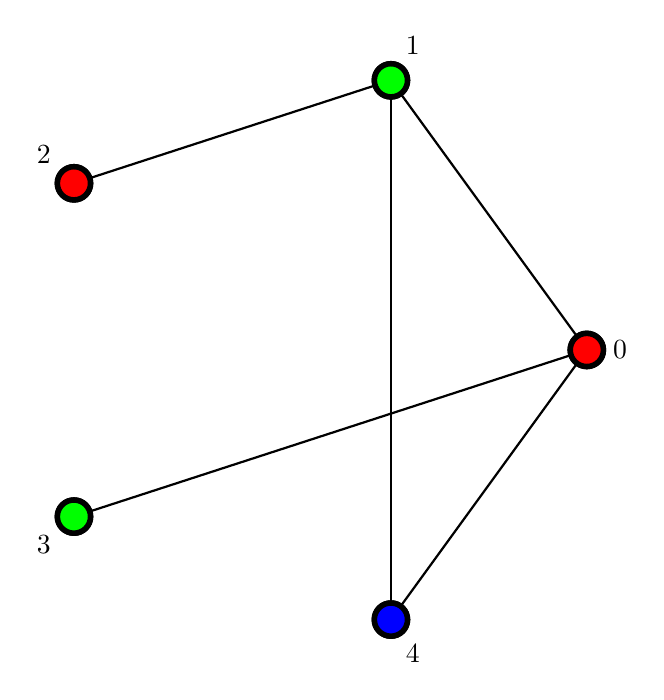
\begin{tikzpicture}[scale=1.2]
\renewcommand*{\VertexLineWidth}{2pt}
\GraphInit[vstyle=Welsh]
\Vertices[unit=3]{circle}{0,1,2,3,4}
\Edges(0,1)
\Edges(0,4)
\Edges(0,3)
\Edges(1,2)
\Edges(1,4)
\SetVertexNoLabel
\AddVertexColor{red}{0}
\AddVertexColor{green}{1}
\AddVertexColor{red}{2}
\AddVertexColor{green}{3}
\AddVertexColor{blue}{4}
\end{tikzpicture}
\caption{TikZ-Graph gerado em Sat Dec 26 00:45:09 2015
.}
\end{figure}
\end{document}
